\documentclass[11pt]{scrartcl}

\usepackage[english]{babel}
\usepackage[utf8]{inputenc}
\usepackage{amsmath}
\usepackage{array}
\usepackage{amsthm}
\usepackage{amssymb}
\usepackage{gensymb}
\usepackage{textcomp}
\usepackage{empheq}
\usepackage{graphicx}
\usepackage{mathtools}
\usepackage[T1]{fontenc}
\usepackage{textcomp}
\usepackage{siunitx}
\usepackage{parskip}
\usepackage{bm}

\title{\textbf{CS 234: Problem Set 1}}
\author{Do-Hyoung Park (dpark027@stanford.edu)}
\date{\today}
\begin{document}
\maketitle

\section*{Problem 1: Bellman Operator Properties}
\subsubsection*{a)}
For any two value functions $V$ and $V'$ such that $V \leq V'$, we have:
$$V(s') \leq V'(s')$$

and since both $V$ and $V'$ are being applied to the same MDP, the probability distributions on the transitions are identical:
$$\bm{E}_{\pi} \bigg[ \gamma \sum_{s' \in S} P(s' \, | \, s,\pi(s)) V(s') \bigg] \leq \bm{E}_{\pi} \bigg[ \gamma \sum_{s' \in S} P(s' \, | \, s,\pi(s)) V'(s') \bigg]$$

and again, since they're being applied to the same MDP, the reward structures are identical:
$$\bm{E}_{\pi} \bigg[R(s, \pi(s)) + \gamma \sum_{s' \in S} P(s' \, | \, s,\pi(s)) V(s') \bigg] \leq \bm{E}_{\pi} \bigg[R(s, \pi(s)) + \gamma \sum_{s' \in S} P(s' \, | \, s,\pi(s)) V'(s') \bigg]$$

which is the same as:
$$\boxed{T_{\pi} V \leq T_{\pi} V'}$$

A similar argument can be used to show that $TV \leq TV'$:
$$V(s') \leq V'(s')$$

since both $V$ and $V'$ are being applied to the same MDP, the probability distributions on the transitions are identical:
$$\gamma \sum_{s' \in S} P(s' \, | \, s,a) V(s') \leq \gamma \sum_{s' \in S} P(s' \, | \, s,a) V'(s')$$

again, since they're being applied to the same MDP, the reward structures are identical:
$$R(s, a) + \gamma \sum_{s' \in S} P(s' \, | \, s,a) V(s') \leq R(s, a) + \gamma \sum_{s' \in S} P(s' \, | \, s,a) V'(s')$$

and since for any $a$ applied to $s$, the corresponding values of $s'$ and the probabilities of those values will be the same, we can say that at the value of $a$ that gives the maximal value of each side, the inequality must also hold:
$$max_{a} \bigg[R(s, a) + \gamma \sum_{s' \in S} P(s' \, | \, s,a) V(s') \bigg] \leq max_{a} \bigg[R(s, a) + \gamma \sum_{s' \in S} P(s' \, | \, s,a) V'(s') \bigg]$$

which shows:
$$\boxed{TV \leq TV'}$$

\subsubsection*{b)}
For any policy $\pi$:
$$T_{\pi} (V + c \vec{1}) = \bm{E}_{\pi} \bigg[ R(s, \pi(s)) + \gamma \sum_{s' \in S} P(s' \, | \, s, \pi(s)) (V(s') + c) \bigg]$$
$$= \bm{E}_{\pi} \bigg[ R(s, \pi(s)) + \gamma \sum_{s' \in S} P(s' \, | \, s, \pi(s)) V(s') + \gamma c \sum_{s' \in S} P(s' \, | \, s, \pi(s)) \bigg]$$
$$= \bm{E}_{\pi} \bigg[ R(s, \pi(s)) + \gamma \sum_{s' \in S} P(s' \, | \, s, \pi(s)) V(s') + \gamma c \bigg]$$
$$= \bm{E}_{\pi} \bigg[ R(s, \pi(s)) + \gamma \sum_{s' \in S} P(s' \, | \, s, \pi(s)) V(s') \bigg] + \bm{E}_{\pi} \bigg[\gamma c \bigg]$$
$$= \bm{E}_{\pi} \bigg[ R(s, \pi(s)) + \gamma \sum_{s' \in S} P(s' \, | \, s, \pi(s)) V(s') \bigg] + \gamma c$$
$$\boxed{= T_{\pi} V + \gamma c \vec{1}}$$

Similarly:
$$T(V + c \vec{1}) = max_{a \in A} \bigg\{R(s,a) + \gamma \sum_{s' \in S} P(s' \, | \, s,a) (V(s') + c) \bigg\}$$
$$= max_{a \in A} \bigg\{R(s,a) + \gamma \sum_{s' \in S} P(s' \, | \, s,a) V(s') + \gamma \sum_{s' \in S} P(s' \, | \, s,a) c \bigg\}$$
$$= max_{a \in A} \bigg\{R(s,a) + \gamma \sum_{s' \in S} P(s' \, | \, s,a) V(s') + \gamma c \bigg\}$$
$$\boxed{= TV + \gamma c \vec{1}}$$

\subsubsection*{c)}
For $\alpha, \beta \geq 0$ and $\alpha + \beta = 1$:
$$T(\alpha V + \beta V') = max_{a \in A} \bigg\{R(s,a) + \gamma \sum_{s' \in S} P(s' \, | \, s,a) (\alpha V(s') + \beta V'(s')) \bigg\}$$
$$= max_{a \in A} \bigg\{R(s,a) + \gamma \alpha \sum_{s' \in S} P(s' \, | \, s,a) V(s') + \gamma \beta \sum_{s' \in S} P(s' \, | \, s,a) V'(s') \bigg\}$$
$$= max_{a \in A} \bigg\{\alpha R(s,a) + \gamma \alpha \sum_{s' \in S} P(s' \, | \, s,a) V(s')\bigg\} + \beta R(s, a) \gamma \beta \sum_{s' \in S} P(s' \, | \, s,a) V'(s') \bigg\}$$
$$\leq max_{a \in A} \bigg\{\alpha R(s,a) + \gamma \alpha \sum_{s' \in S} P(s' \, | \, s,a) V(s')\bigg\} + max_{a' \in A} \bigg\{\beta R(s,a') + \gamma \beta \sum_{s' \in S} P(s' \, | \, s,a') V'(s')\bigg\}$$ 
$$= \alpha \, max_{a \in A} \bigg\{R(s,a) + \gamma \sum_{s' \in S} P(s' \, | \, s,a) V(s')\bigg\} + \beta \, max_{a' \in A} \bigg\{R(s,a') + \gamma \sum_{s' \in S} P(s' \, | \, s,a') V'(s')\bigg\}$$
$$= \alpha TV + \beta TV'$$

Thus, $T(\alpha V + \beta V') \leq \alpha TV + \beta TV'$.

\subsubsection*{d)}
This statement is \fbox{false}.

Consider an example in which $V(s) = 0$ for $\forall s \in S$ with $\gamma = 0$ and $R(s,a) = 1$ for $\forall a \in A, \forall s \in S$. In this case:
$$(TV)_{(s)} = max_{a \in A} \bigg\{R(s,a) + \gamma \sum_{s' \in S} P(s' \, | \, s,a) V(s') \bigg\}$$
$$= 1$$

for all $s$, while $V(s) = 0$ for all $s$, as defined in the problem. Thus, it is not always true that $TV \leq V$.
 
\section*{Problem 2: Value Iteration}
\subsubsection*{a)}
Yes, the policy can change again in such a scenario. Take, for example, a simplified version of the Mars rover given as an example in class, in which there are four states, $S_1, S_2, S_3, S_4$, in a row in a one-dimensional world, and our rover can take two actions, ``move left'' and ``move right,'' which are deterministic (that is, will achieve the desired action with probability $1$). Say that $S_1$ has a reward of $+10$ and $S_4$ has a reward of $+1000$, while $S_2, S_3$ have reward $0$.

Doing value iteration with $\gamma = 1$ gives us the following values for the states at each iteration: $(0,0,0,0) \to (10,0,0,1000) \to (20,10,1000,2000) \to (30,1000,2000,3000)$. It's clear that in the second and third step, the optimal policy at $S_0$ is to take ``move left,'' but in the fourth step, the optimal policy at $S_0$ is to take ``move right.''

\subsubsection*{b)}
\emph{This proof was originally presented by Singh, S. and Yee, R. in their paper ``An Upper Bound on the Loss from Approximate Optimal-Value Functions.''}

\emph{Incidentally, after having devoted a full day to this problem and then finding the proof online, I don't think I could have derived this myself even if I'd been given an extra week.}

Consider there to be a state $z$ at which the loss function $L_{\tilde{V}}(s)$ is at a maximum; that is, $L_{\tilde{V}}(z) \geq L_{\tilde{V}}(s)$ for $\forall{s} \in S$. At state $z$, consider two policies $a = \pi^{*}(z)$, which would be the optimal policy from state $z$, and $b = \pi_{\tilde{V}}(z)$, which is the greedy policy derived from our value estimate $\tilde{V}$. This means that $Q_{\tilde{V}}(z,a) \leq Q_{\tilde{V}}(z,b)$, since the greedy policy will always take the policy with the highest $Q$-value, regardless of whether or not it is the actual optimal policy.
$$Q_{\tilde{V}}(z,a) \leq Q_{\tilde{V}}(z,b)$$
$$R(z, a) + \gamma \sum_{s' \in S} p(s' \, | \, a,z)\tilde{V}(s') \leq R(z, b) + \gamma \sum_{s' \in S} p(s' \, | \, b,z)\tilde{V}(s')$$

We now assert that since $\vert V^{*}(s) - \tilde{V}(s) \vert \leq \epsilon$ for all $s$:
$$V^{*}(s') - \epsilon \leq \tilde{V}(s') \leq V^{*}(s') + \epsilon$$

which, combining with our earlier result, yields:
$$R(z, a) + \gamma \sum_{s' \in S} p(s' \, | \, a,z)[V^{*}(s') - \epsilon] \leq R(z, b) + \gamma \sum_{s' \in S} p(s' \, | \, b,z)[V^{*}(s') + \epsilon]$$
$$R(z, a) + \gamma \sum_{s' \in S} p(s' \, | \, a,z)V^{*}(s') - \epsilon \gamma \leq R(z, b) + \gamma \sum_{s' \in S} p(s' \, | \, b,z)V^{*}(s') + \epsilon \gamma$$
$$R(z, a) - R(z, b) \leq \gamma \sum_{s' \in S} \bigg( p(s' \, | \, b, z) V^{*}(s') - p(s' \, | \, a, z) V^{*}(s') \bigg) + 2 \epsilon \gamma$$

Since state $z$ is the state at which the loss function is maximized, the loss function computed at $z$ is the upper bound of the loss function:
$$L_{\tilde{V}}(z) = V^{*}(z) - V_{\pi_{\tilde{V}}} (z)$$
$$= R(z,a) + \gamma \sum_{s' \in S} p(s' \, | \, a,z) V^{*}(s') - R(z,b) - \gamma \sum_{s' \in S} p(s' \, | \, b,z) V_{\pi_{\tilde{V}}}(s')$$
$$= R(z,a) - R(z,b) + \gamma \sum_{s' \in S} \bigg[ p(s' \, | \, a,z) V^{*}(s') - p(s' \, | \, b,z) V_{\pi_{\tilde{V}}}(s') \bigg]$$

Combining with the inequality from above:
\begin{multline*}
L_{\tilde{V}}(z) \leq \gamma \sum_{s' \in S} \bigg( p(s' \, | \, b, z) V^{*}(s') - p(s' \, | \, a, z) V^{*}(s') \bigg) + 2 \epsilon \gamma \\
+ \gamma \sum_{s' \in S} \bigg[ p(s' \, | \, a,z) V^{*}(s') - p(s' \, | \, b,z) V_{\pi_{\tilde{V}}}(s') \bigg]
\end{multline*}
$$= \gamma \sum_{s' \in S} p(s' \, | \, b,z) \bigg( V^{*}(s') - V_{\pi_{\tilde{V}}}(s') \bigg) + 2 \epsilon \gamma$$
$$= \gamma \sum_{s' \in S} p(s' \, | \, b,z) L_{\tilde{V}}(s') + 2 \epsilon \gamma$$
$$\leq \gamma \sum_{s' \in S} p(s' \, | \, b,z) L_{\tilde{V}}(z) + 2 \epsilon \gamma$$
$$L_{\tilde{V}}(z) \leq \gamma L_{\tilde{V}}(z) + 2 \epsilon \gamma$$
$$L_{\tilde{V}}(z) (1 - \gamma) \leq 2 \epsilon \gamma$$
$$\boxed{L_{\tilde{V}}(z) \leq \frac{2 \epsilon \gamma}{1 - \gamma}}$$

\section*{Problem 3: Grid Policies}
\subsubsection*{a)}
First, let us note that:
$$Q^{*}(s,a) = r(s,a) + \gamma \sum_{s' \in S} p(s' \, | \, a,s) V^{*}(s')$$

and:
$$V^{*}(s) = max_{a} Q^{*}(s,a)$$

and:
$$\pi^{*}(s,a) = argmax_{a} Q^{*}(s,a)$$

Since we take the transitions to be deterministic and $\gamma = 1$ in this problem, this simplifies to:
$$Q^{*}(s,a) = r(s,a) + \gamma V^{*}(s')$$

There are going to be three types of transitions in this problem: Those that bring us closer to the goal, those that take us further away from the goal, and those that do neither (e.g. hit a wall, in which case we remain in the same place). We want to assign reward values such that the actions that bring us closer to the goal are chosen every time. It is easily gathered that $V^{*}(11) = 5$ and $V^{*}(15) = -5$ based on their rewards and their statuses as terminal states.

Let's take the action from state 12 as an example. We have four separate actions, for which we can represent $Q$-values as follows:
$$Q^{*}(12,L) = r(12,L) + V^{*}(11)$$
$$Q^{*}(12,U) = r(12,U) + V^{*}(17)$$
$$Q^{*}(12,D) = r(12,L) + V^{*}(12)$$
$$Q^{*}(12,R) = r(12,R) + V^{*}(13)$$

Of these, the uppermost action is the desired one, and thus we want that to have the highest $Q$-value. If we take the reward for this action to be $r(12,L) = +1$, then we see that $Q^{*}(12,L) = 6$, meaning that $V^{*}(12) = 6$. In general, this will mean that the optimal value for each square will increase by one as we get one space ``further away'' from the goal state. That is, $V^{*}(13) = V^{*}(17) = 7$, and so on. However, this will mean that the undesirable action $(12,R)$ can only have $Q$-value at minimum $Q^{*}(12,R) = -1 + 7 = 6$, which is equal to the $Q$-value for our desired action. Thus, in this case, we can't be guaranteed that our ideal policy will be taken. Thus, the reward for our desired action cannot be $+1$.

If we take the reward for the desired action to be $r(12,L) =  -1$, then we have $Q^{*}(12,L) = V^{*}(12) = 4$, meaning that the optimal value fo each square will decrease by one as we get one space ``further away'' from the goal state. Thus, $V^{*}(13) = V^{*}(17) = 3$ and so on. If we choose the reward for all ``undesired'' actions to be $-1$, we're guaranteed to get our desired action every time, as in this case, $Q^{*}(12,R)=Q^{*}(12,U)=2$ and $Q^{*}(12,D)=3$.

Finally, if we take the reward for the desired action to be $r(12,L) = 0$, then we have $Q^{*}(12,L) = V^{*}(12)=5$, meaning that all squares will have optimal value of $5$ (if we extend this logic to all squares). As long as we take the reward for all ``undesired'' actions to be $-1$, we're guaranteed to get our desired action every time, as in this case, $Q^{*}(12,R)=Q^{*}(12,U)=Q^{*}(12,D)=4$. Since this reward structure gives us higher values of $V^{*}(s)$ across the states, we choose this reward structure over the former one.

Thus, we define $r(s,a) = 0$ when taking action $a$ from state $s$ moves us closer to state $11$, and $r(s,a) = -1$ for all other action-state combinations outside of the goal states.

\subsubsection*{b)}
As stated in the previous section, we have $V^{*}(11) = +5$, $V^{*}(15) = -5$, and $V^{*}(s) = +5$ for all other states.

\subsubsection*{c)}
With this reward structure, setting $\gamma = 0.5$ will not change the optimal policy since all values of $V^{*}(s)$ are equal (outside of state 15, which will never be chosen anyway). Changing $\gamma$ only changes how much the $V^{*}$ values are weighted, but won't change the reward structure, which is the only factor that determines our optimal policy.

\subsubsection*{d)}
The optimal value function will change so that $V^{*}(s) = +20$ for all states outside of state $15$, for the reasons outlined in part a). The policy won't change, either, since the optimal policy is only dictated by the reward structure when all states have identical $V^{*}$.

\section*{Problem 4: Frozen Lake MDP}
\subsubsection*{c)}
Stochasticity is seen to greatly increase the number of iterations required. In a deterministic world, the policy and value iterations would reliably converge within 4-7 iterations for my selected hyperparameters, but in the stochastic world, the pre-set $20$ iterations wouldn't be enough to achieve convergence. The resulting policy seems to rely much more on taking advantage of chance to move towards the goal state instead of actively steering towards it. I presume this might be because the optimal policy tries to keep the player away from states that border a hole, as the stochastic world offers a chance of misstepping and failing with reward $0$ whenever the player is adjacent to a hole, which would incentivize the program to try to keep the player away from those hole-adjacent states as much as possible.

\begin{center}
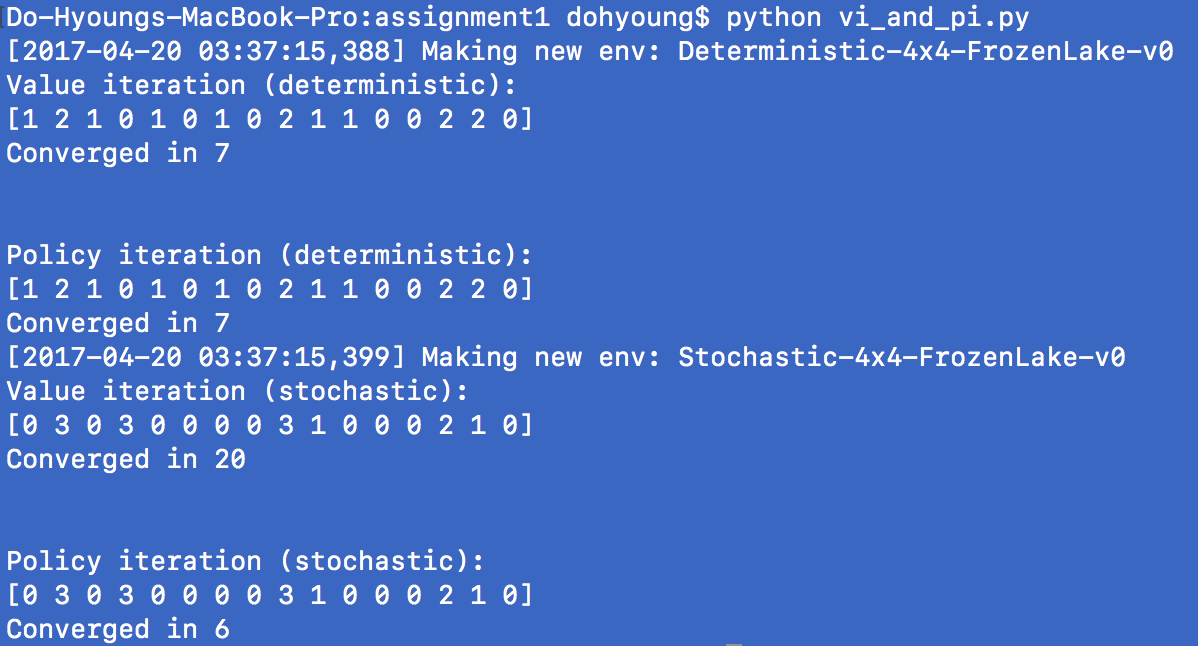
\includegraphics[width=\textwidth]{PS1Q4.png}
\end{center}

\section*{Problem 5: Frozen Lake Reinforcement Learning}
\subsubsection*{c)}
\begin{center}
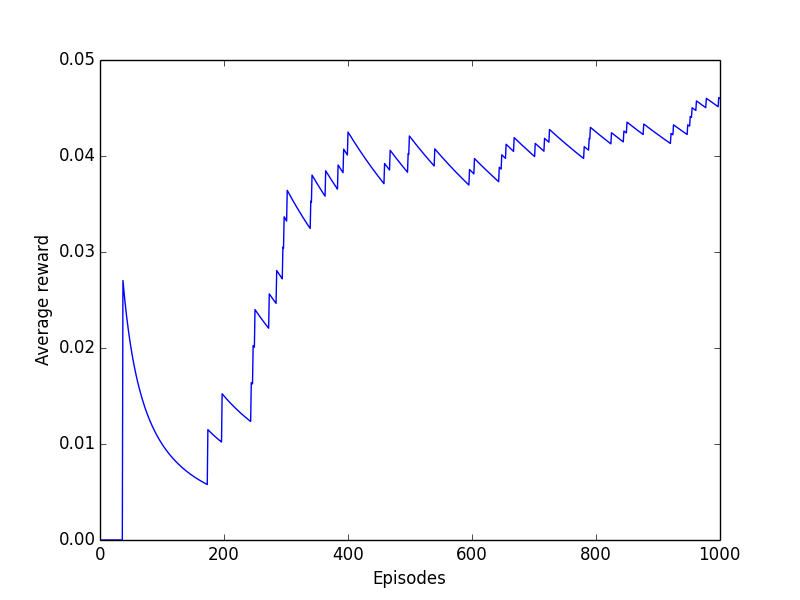
\includegraphics[width=\textwidth]{PS1Q5c.png}
\end{center}

\subsubsection*{d)}
\begin{center}
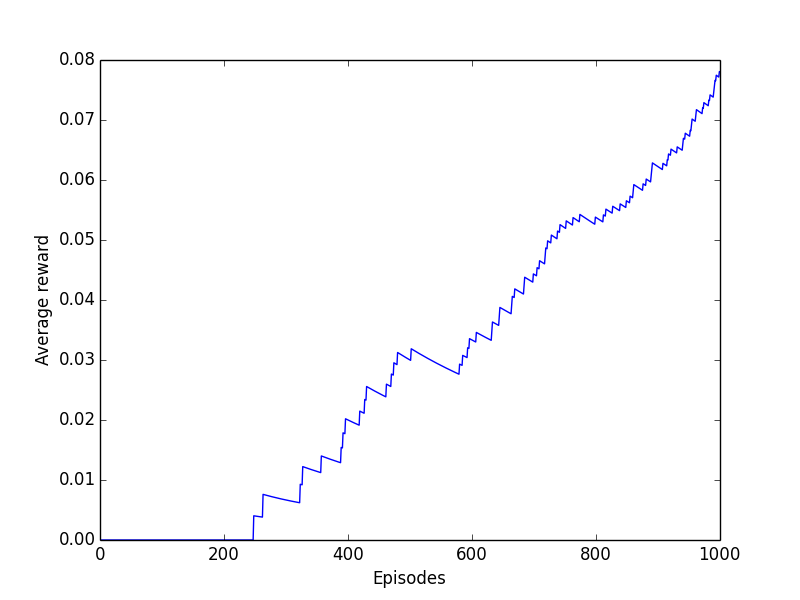
\includegraphics[width=\textwidth]{PS1Q5d.png}
\end{center}

One benefit of Q-learning seems to be that it can be done much more efficiently than model-based learning, as it doesn't require the computationally intensive value iteration step at the start of every episode like model-based learning does, and updating a $Q$ matrix is also more computationally efficient than having to deal with and update a messy dictionary in every episode like in model-based learning. A benefit of model-based learning, though, is that we do end up learning about our environment and its model parameters in the limit of a large number of training episodes, which ends up being useful for use in value and policy iteration to gain better policy estimates than with Q-learning.

\end{document}